\chapter{Caracteristicas de transferencia de Corriente}
    Las \textbf{características de transferencia de corriente} del transistor BJT describen la relación entre la corriente de base $I_B$ y la corriente de colector $I_C$, manteniendo constante la tensión colector-emisor $V_{CE}$. Esta relación es clave en la región activa del transistor, donde éste funciona como amplificador de corriente.
    
    En dicha región, se cumple la relación:
    
    \[
    I_C = \beta \cdot I_B
    \]
    
    donde $\beta$ (también conocido como $h_{FE}$) representa la ganancia de corriente continua del transistor en configuración emisor común. Esta relación es aproximadamente lineal para un amplio rango de operación y es la base del comportamiento amplificador del BJT.
    
    El estudio experimental de estas características permite determinar el valor de $\beta$ y observar cómo varía con $I_B$, facilitando la comprensión del funcionamiento interno del transistor y su comparación con el modelo teórico.

\newpage

  \section{Simulacion}

  En esta etapa se realiza la simulación del circuito para obtener la curva $I_C$ vs.\ $I_B$, con $V_{CE}$ constante. Se utiliza una barrida de corriente de base para analizar el comportamiento del transistor y estimar su ganancia de corriente continua $\beta$.

  %Circuito usado en la simulacion
  %Grafico de la simulacion

\newpage

  \section{Laboratorio}

  Se realizan mediciones experimentales de $I_C$ en función de $I_B$ con tensión $V_{CE}$ fija, replicando condiciones similares a las de la simulación. Esto permite comparar el modelo teórico del BJT con su comportamiento real en laboratorio.

  Debido a que el circuito a analizar es el mismo que el ejercicio anterior se muestran imagenes de donde se va a realizar la medicion:
  \begin{figure}[!ht]

        \begin{minipage}{0.5\textwidth}
            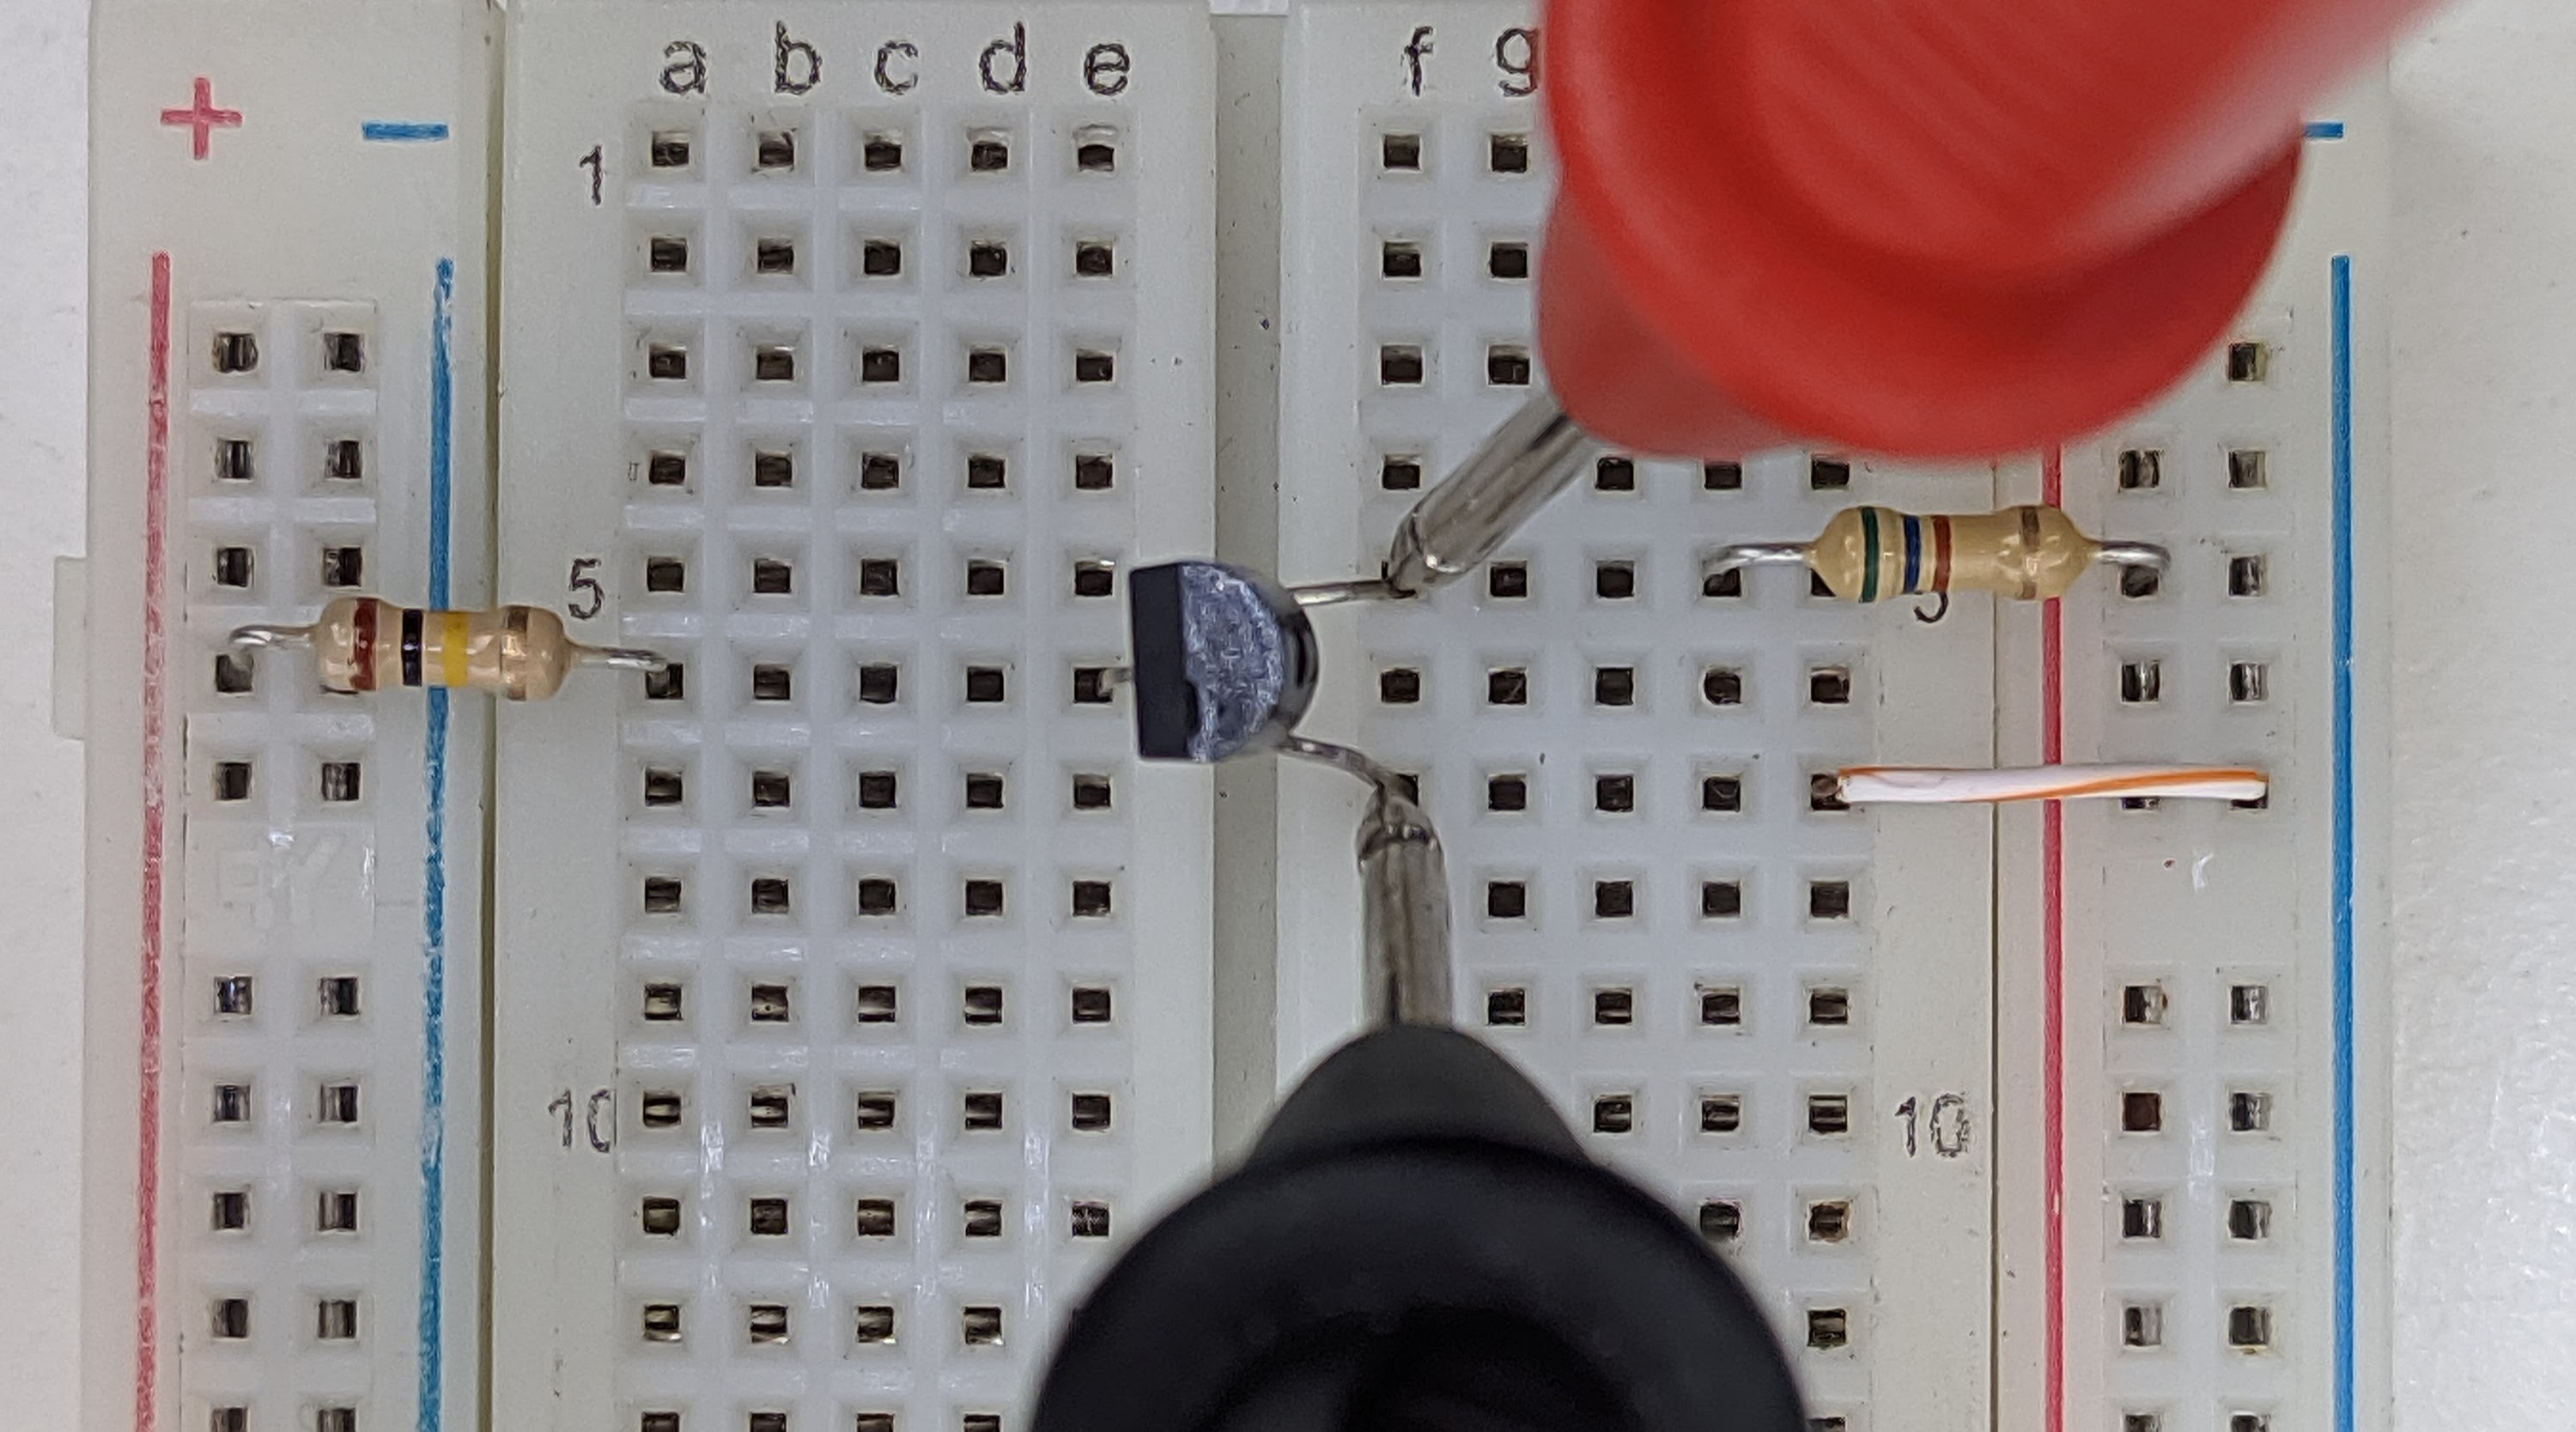
\includegraphics[width=1\textwidth]{tp3/pictures/prot_crkt-3_Vce.jpg}
            \caption{Mediciones de $V_{CE}$.}
 
        \end{minipage}
                    \begin{minipage}{0.5\textwidth}
            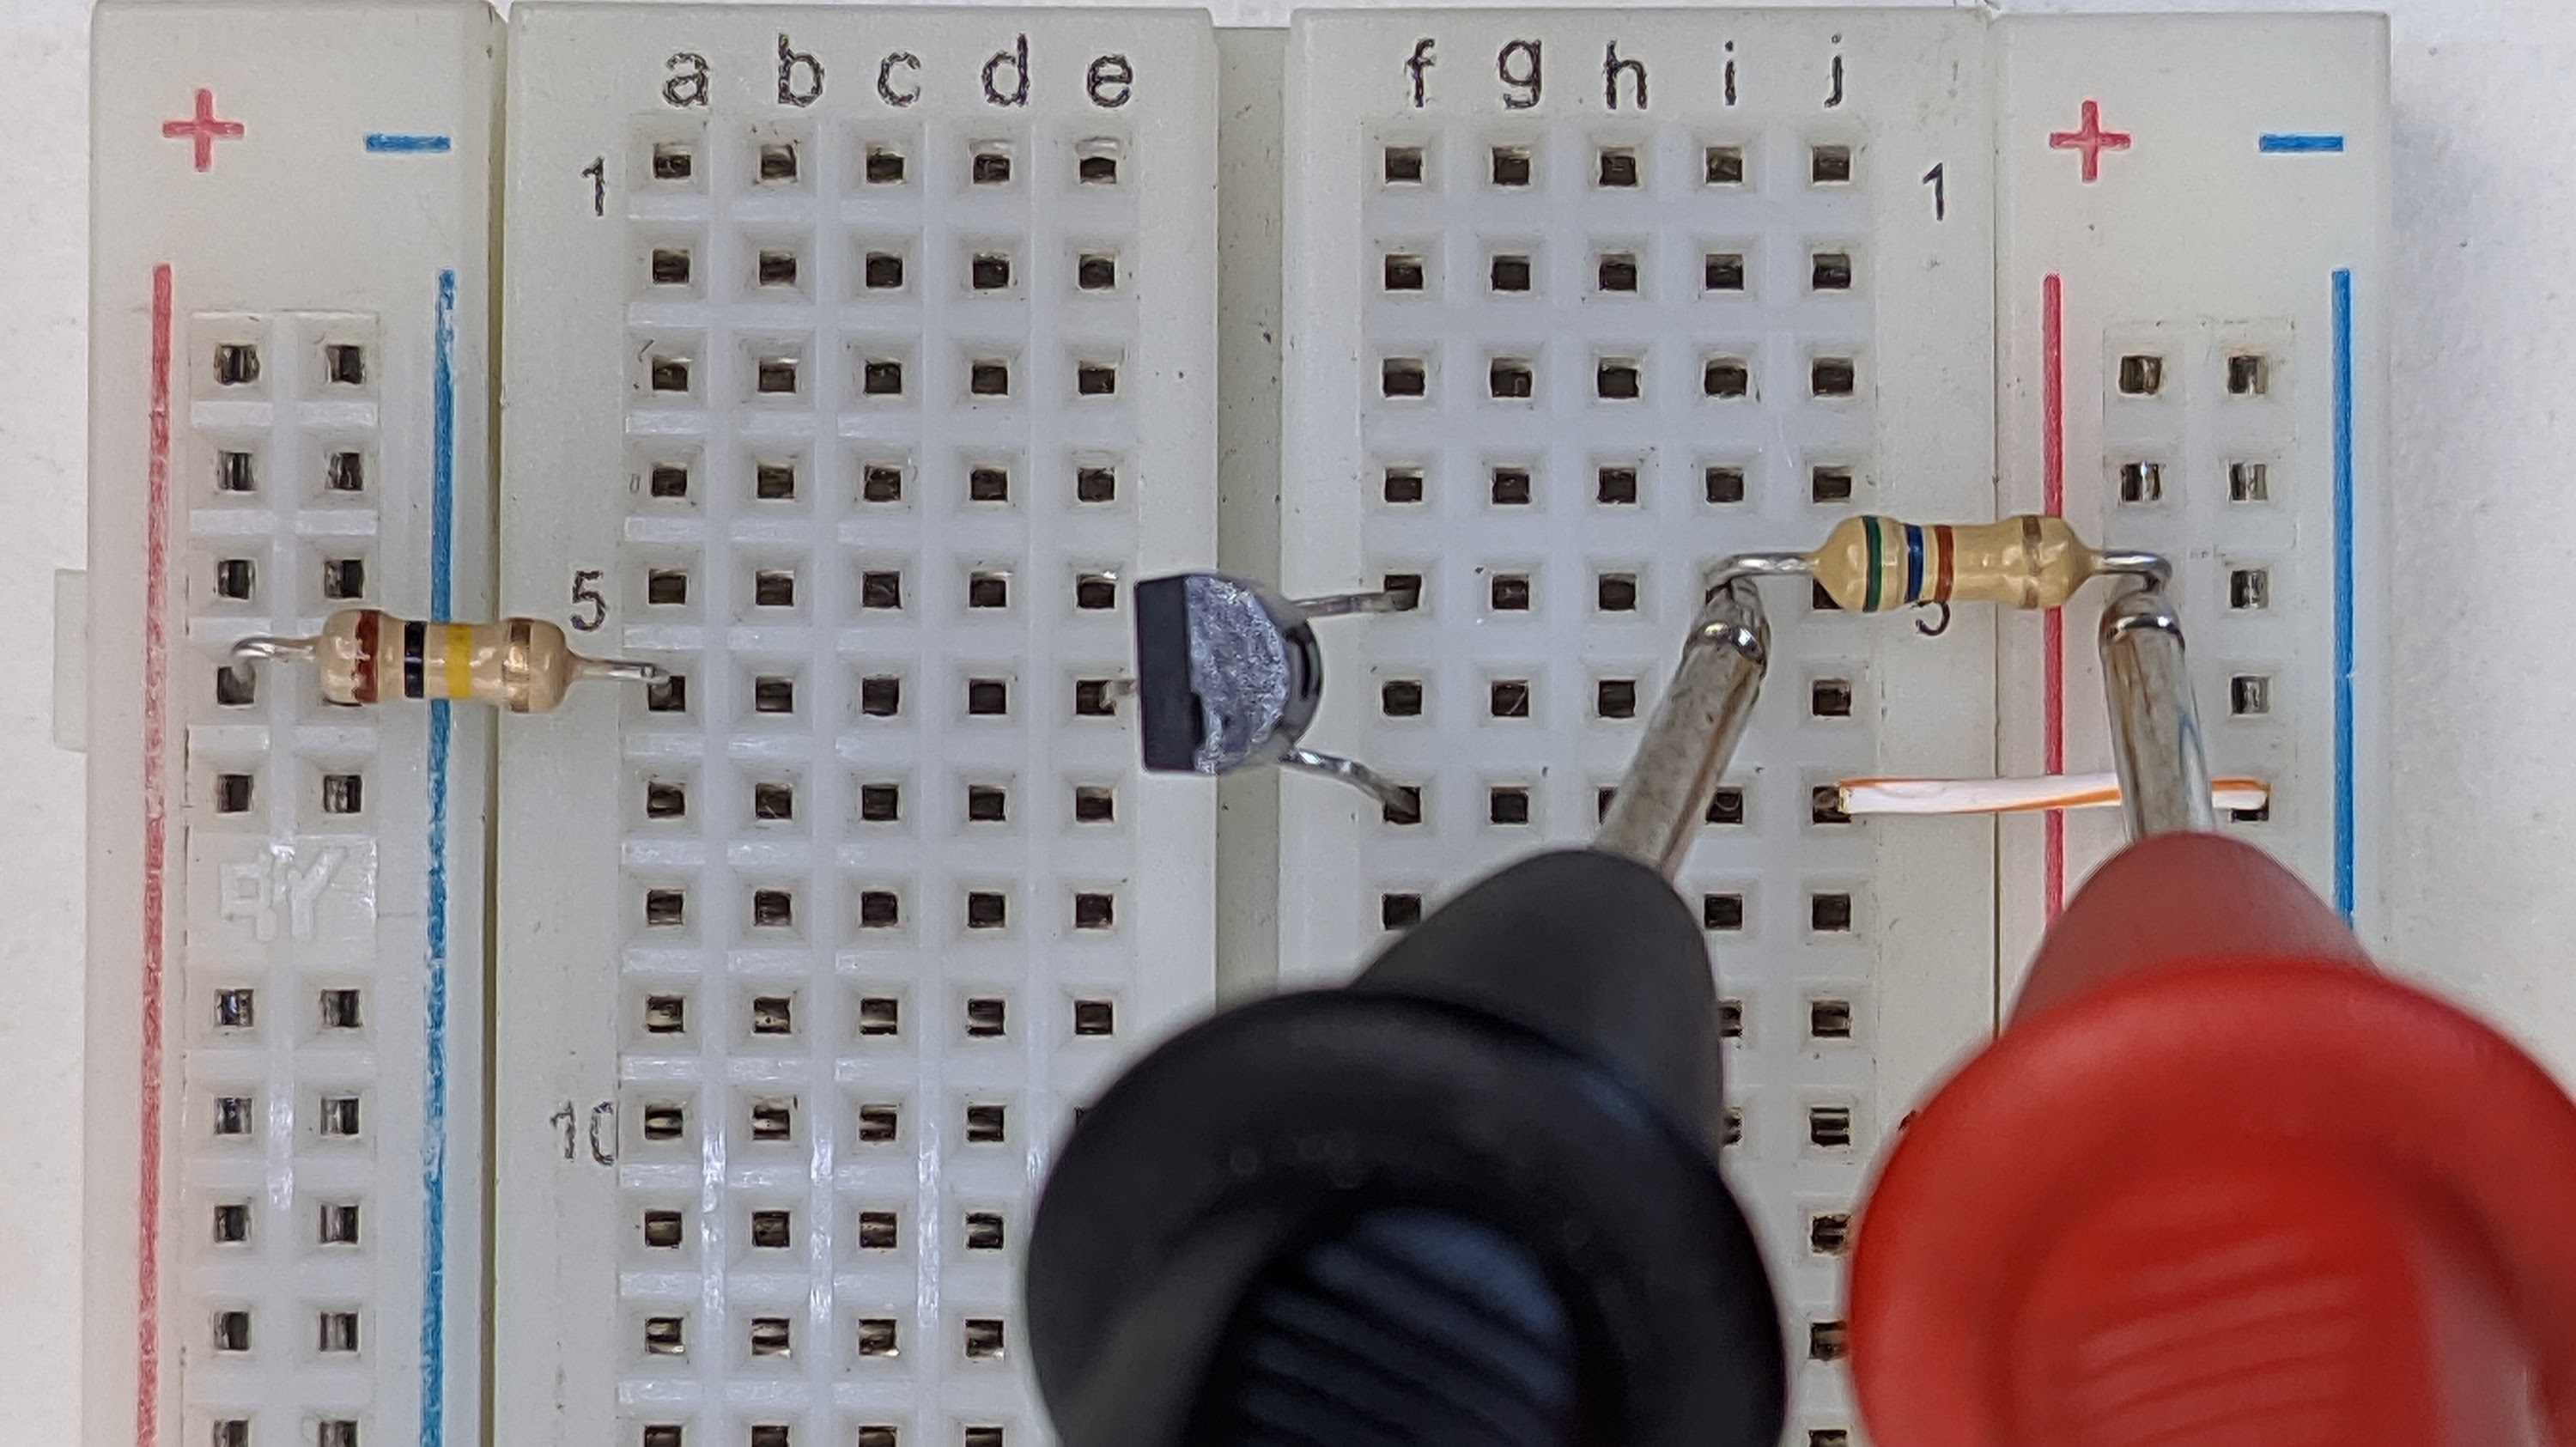
\includegraphics[width=1\textwidth]{tp3/pictures/prot_crkt-3_Vrc.jpg}
            \caption{Mediciones de $V_{RC}$.}

        \end{minipage}
        
 
    \end{figure}

    Se presenta el cuadro con las medidas obtenidas:

     \begin{table}[h!]
    \centering
    \small 
    \begin{tabular}{|c|c|c|c|}
    \hline
    $I_B$ [$\mu$A] & $I_C$ ($V_{CE} = 2\,V$) & $I_C$ ($V_{CE} = 5\,V$) & $I_C$ ($V_{CE} = 8\,V$) \\
    \hline
    5  &           &           &           \\
    \hline
    7  &           &           &           \\
    \hline
    10 &           &           &           \\
    \hline
    20 &           &           &           \\
    \hline
    \end{tabular}
    \caption{Corriente de colector medida para distintos valores de $V_{CE}$ e $I_B$ constantes.}
    \end{table}  
    \caption{Mediciones de $I_B$ y $V_{BE}$ para diferentes valores de $V_{BB}$. Valores de$I_B$ estimados según el comportamiento exponencial típico de la unión BE.}


\newpage

 \section{Conclusion}

    En esta sección se analizó la relación entre la corriente de colector $I_C$ y la corriente de base $I_B$ con $V_{CE}$ constante, lo que permitió obtener la característica de transferencia del transistor BJT. Tanto en simulación como en laboratorio se observó un comportamiento creciente y aproximadamente lineal entre ambas corrientes en la región activa, lo que permitió calcular la ganancia de corriente continua $\beta$ del dispositivo.

    Los resultados experimentales mostraron que pequeñas variaciones en $I_B$ generan cambios significativos en $I_C$, confirmando la función del BJT como amplificador de corriente. La concordancia entre los valores simulados y medidos validó el modelo teórico, destacando la importancia de esta característica para el diseño y análisis de circuitos con transistores.
